\nsection{Alpine Hashing}
\label{ex:alpine}

Here we look at a cache-coherent, open-addressing hashtable structure
which lends itself to speed-up using SIMD vector operations.
It's somewhat similar in concept to Google's \verb^Swiss Table^:
\wwwurl{https://abseil.io/about/design/swisstables}

\noindent
Every key is used to generate a $32$-bit hash, which is decomposed into
two parts.  The top $25$-bits ($h_1$) are used (before modulo arithmetic)
to compute which `bucket' the key/value pair will be stored into, and
the remaining $7$-bits ($h_2$) are used as a `fingerprint' to enable
fast lookup.

Each bucket is filled from the front, probing right until an empty slot is found. You skip over tombstoned slots.
If a bucket becomes full, insertion continues in the next bucket along.


\begin{figure}[ht]
\centering{
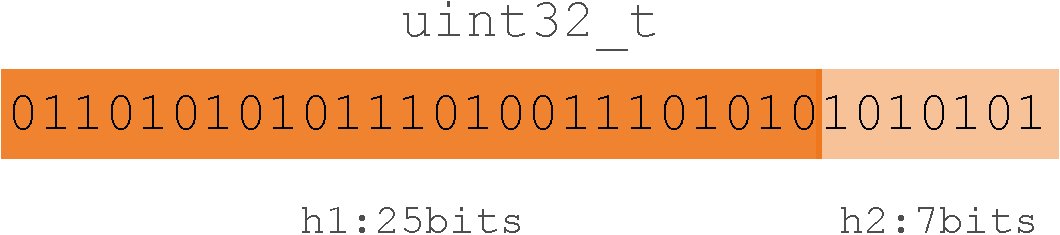
\includegraphics[clip,width=1.00\textwidth,page=1]{../Pictures/alpinehash.pdf}
}
\caption{The Alpine Hashtable master hash, decomposed into $h_1$ and $h_2$.} 
\label{fig:ahash}
\end{figure}

\noindent
Each bucket consists of (usually) $16$ slots, each of which has space
for a key, its value, and a control byte. This control byte has its top
bit set to zero for a valid entry, or set to one if the slot is empty
or has been deleted (tombstoned). For a valid entry the control byte has
a zero top bit and the remaining bits are the corresponding $h_2$ bits.

\noindent
This h$_2$ hash can be used as quick check as to whether that key exists
in the bucket, but since these are only $7$ bits, a further deep check
comparing the two keys in question is required if the two $h_2$ hashes match.

\noindent
The number of buckets varies, typically increasing when the loading (number
of cells in use) becomes too large, or shrinking when it becomes too low.


\begin{figure}[ht]
\centering{
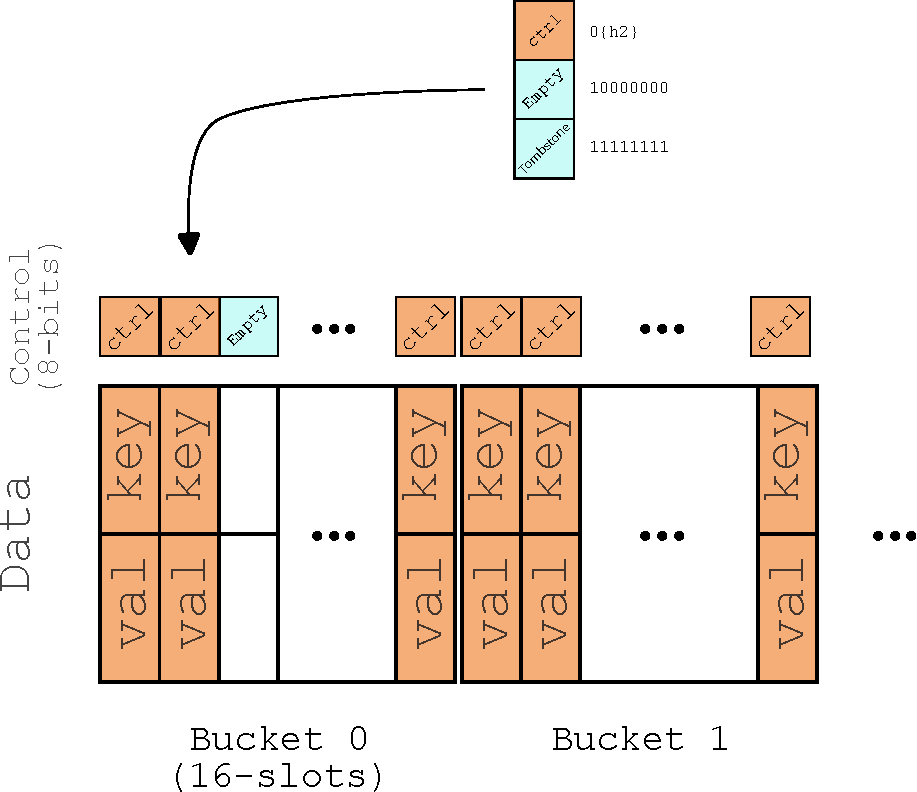
\includegraphics[clip,width=1.00\textwidth,page=1]{../Pictures/alpinestruct.pdf}
}
\caption{The Alpine Hashtable layout, with a single, large array of data buckets (each containg $16$ slots), and
a corresponding array of control-bytes.}
\label{fig:ahash}
\end{figure}

\begin{exercise}
Write an ADT to implement the \verb^ahash.h^ given.  Write the
source file \verb^ahash.c^ such that
the driver file \verb^driver.c^
work correctly.  Ensure that this all works with my \verb^Makefile^
which {\bf must be} used {\bf unaltered}.  The basic operations are~:
\begin{verbatim}
ahash* ahash_init(uint32_t (*f)(const char *str));
bool ahash_insert(ahash** a, const char* key, const char* val);
bool ahash_isin(const ahash* a, const char* key, char* val);
bool ahash_delete(ahash** a, const char* key);
void ahash_free(ahash** a);
\end{verbatim}

\noindent
and an optional/extension function~:
\begin{verbatim}
char* ahash_ctrl(const ahash* a, char* ret);
\end{verbatim}

\noindent more information is given in the header file, but in summary~:

\noindent \verb^ahash_init()^ initialises the structure
with a function pointer to the hash function used throughout.

\noindent \verb^ahash_insert()^ returns a Boolean showing whether
an insertion has been possible. Since the table might be resized you
pass a pointer to a pointer, so that if the memory allocation changes,
the original pointer is still valid.

\noindent \verb^ahash_isin()^ returns Boolean a stating whether or not the
key is found in the table. If it is, the value is copied into \verb^val^.

\noindent \verb^ahash_delete()^ returns whether the key can be found in the table,
and if so, sets its control key to be the `tombstone' flag. Again,
since the table may be resized if the table becomes too sparse, a double
pointer is used for the \verb^ahash^ data structure.

\noindent \verb^ahash_free()^ frees up all memory allocated, and sets
the original pointer to \verb^NULL^.

\noindent
The optinal (extension) function \verb^ahash_ctrl()^ copies a compact
summary of the top-bits (only) of control bytes for the table into the
string \verb^ret^ and returns a pointer to this string, or else returns
\verb^NULL^.

Soem hints and tips~:

\begin{itemize}

\item Even if you don't get all the functions to work correctly, make
sure the code still compiles by writing `dummy' functions as placeholders,
even if some of the assertions fail.

\item  This assignment is brand new. If minor typos etc. are uncovered
as you complete the assignment we may update this documentation and/or
the online files provided. Please check regularly to make sure you are
using the most recent version.

\item Do no printing as part of \verb^ahash.c^ - the driver will do any printing required.

\end{itemize}

\noindent {\bf This is worth $90\%$ of the marks.}
\vspace*{1ex}

\noindent
Two extensions are available, each worth $5\%$.

\noindent The \verb^ahash_ctrl()^ fucntion described above. I'll
test whether you've completed this extension by running the examples
given in the driver (and others).

\noindent A second extension, to implement a faster means of checking for
the presence of matching $h_2$ bytes (and empty slots) using SIMD/AVX
functions.  I haven't really covered this in detail, so would expect
this to be self-taught.  For reference, my implementation used functions
including  \verb^_mm_set1_epi8()^ and \verb^mm_cmpeq_epi8()^. You can
assume that the buckets are a fixed number of slots (16).  A typical
implementation will make operations on the table faster, but only by
$~20\%$ or so?

\noindent
To help with this, make alterations to your code in the original \verb^ahash.c^ file
so that when the \verb^AVX^ flags are enabled via the compiler, differnt code is
compiled, e.g.
\begin{verbatim}
#ifdef __AVX__
   // Do it the fast way
#else
   // Compare the standard way, one byte at a time.
#endif
\end{verbatim}

\end{exercise}
